\documentclass[12pt,journal,onecolumn]{IEEEtran}

%% ** Style Notice **
%% **Different IEEE style can be chosen by changing \documentclass[12pt,journal,onecolumn]{IEEEtran} to \documentclass[12pt,conference,onecolumn] and etc.
%% ** For detail info please visit IEEE_Original folder and check IEEEtran_HOWTO.pdf
%% ** One Column style with normal font of 12 pt is set, delete onecolumn in doucumentclass if you need double column
%% ** Style is mainly based on IEEEtrans template and if you want to change different line distance or font scale, check IEEEtran_HOWTO.pdf
%% ** Tested in Microsoft Visual Studio Code, with Latex-Workshop extension, texlive2018 environment installed. No guarantee on other platform (linux or mac) or other tex environment.

%% ** 这个不是天大毕业论文模板,应付普通大作业/结课报告用的
%% ** 此模板图,表,章节标题默认中文
%% ** 模板基于IEEEtran
%% ** 其实看着很奇怪,就凑合这样了
%% ** 其实只用封皮就可以了---溜走
%% ** github已有很多天大中文的毕业论文模板,要想用比较符合中文的报告模板可以直接拿来用了
%% ** 字号,行间距,缩进等修改请仍然参考IEEEtran_HOWTO.pdf
%% ** 模板没有对IEEEtran.cls修改(patchcmd很好用)
%% ** IEEE模板有很多样式,journal, conference等,可以更改第一行\documentclass参数来修改,参考IEEEtran_HOWTO.pdf(比如conference的页码就在底部)
%% ** 编辑环境为Windows+VSCode+Latex-Workshop extension+texlive2018,已知mac和linux中文显示会跟Windows不同,控制序列\songti不可用,不保证其他平台可用性....请参考ctex手册对照自己平台修改...

\usepackage[pdftex]{graphicx}
\DeclareGraphicsExtensions{.pdf,.jpeg,.png,.eps}
\usepackage{svg}
\usepackage{epstopdf}
\usepackage{cite}
\usepackage{amsmath}
\usepackage{algorithmic}
\usepackage{array}
\usepackage{amsfonts,amssymb}
\usepackage{textcomp}
\ifCLASSOPTIONcompsoc
 \usepackage[caption=false,font=normalsize,labelfont=sf,textfont=sf]{subfig}
\else
 \usepackage[caption=false,font=footnotesize]{subfig}
\fi
\usepackage{url}
\usepackage[hidelinks]{hyperref}

\usepackage[UTF8,scheme=chinese]{ctex} % Add support for Chinese characters.

% \usepackage[english]{babel} % Incase you have some special french or other characters in your bib and main tex. Comment out if you don't need. English Environment

\usepackage{caption} % Reduce the space after caption.
\captionsetup{font=scriptsize}
\setlength\belowcaptionskip{-8pt}

\usepackage[autostyle]{csquotes} %Resolve quotation mark  direction problems.
\MakeOuterQuote{"} % English Environment only

\usepackage{etoolbox} % Use patchcmd to control alignment of section title.

\hyphenation{semi-conduc-tor} % Avoid unwanted hyphenation.


\begin{document}

% this is the Cover
\begin{center}
  \quad
  
  \vspace{1cm}

  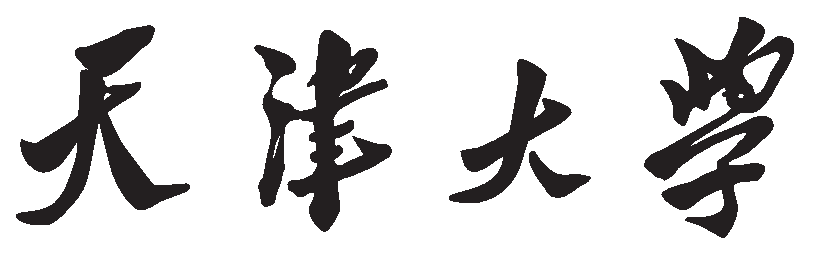
\includegraphics[width=7cm]{./logo/TDFonts.eps}
  \vspace{1cm}


  {
  \fontfamily{phv}
  \fontsize{24}{30}
  \selectfont \textbf{SAMPLE TITLE HERE}
  }

  \vspace{1cm}
  
\includegraphics[width=5.5cm]{./logo/TDLogo.eps}
  \vspace{5cm}

  %% ** Warning::
  %% ** The following \songti control sequence only works on Windows, Linux and mac platform please comment it out
  \begin{table}[h!]
    \centering
    \label{tab:authorinfo}
    \fontsize{16}{30}
    \selectfont
    \begin{tabular}{cl}
    {\songti \textbf{学\ \ \ \ 院:}} & {\songti  \textbf{************学院\ \ }} \\ \cline{2-2}
    {\songti \textbf{专\ \ \ \ 业:} }& {\songti \textbf{************}}\\ \cline{2-2}
    {\songti \textbf{姓\ \ \ \ 名:} }& {\songti \textbf{** ****}}\\ \cline{2-2}
    {\songti \textbf{学\ \ \ \ 号:}} & {\songti \textbf{1234567890}}\\ \cline{2-2}
    \end{tabular}
  \end{table}
  {\fontsize{14}{20}
  \selectfont 2019年12月16日}
  
\end{center}
  \thispagestyle{empty}
  \setcounter{page}{0}
  \clearpage

\title{\textbf{SAMPLE TITLE}}

%% Author information 
% \author{Michael~Shell,~\IEEEmembership{Member,~IEEE,}
%         John~Doe,~\IEEEmembership{Fellow,~OSA,}
%         and~Jane~Doe,~\IEEEmembership{Life~Fellow,~IEEE}% <-this % stops a space
% }


% \thanks{M. Shell was with the Department
% of Electrical and Computer Engineering, Georgia Institute of Technology, Atlanta,
% GA, 30332 USA e-mail: (see http://www.michaelshell.org/contact.html).}% <-this % stops a space


%% This section changes the Footer and Header of page
\markboth{页眉示例}% even 
{页眉示例} % odd
\maketitle

%% Abstract here if you want write abstract, comment it out.
% \begin{abstract}
%   The abstract goes here.
% \end{abstract}

%% Keyword, comment out before use.
% \begin{IEEEkeywords}
%   IEEE, IEEEtran, journal, \LaTeX, paper, template.
% \end{IEEEkeywords}

\patchcmd{\section}{\centering}{\raggedright}{}{} % Change default IEEE template centering section title to align left
\patchcmd{\section}{\normalsize}{\large\bfseries}{}{} % Change Title to large Boldface

\section{绪论}

"The Islands of Tahiti are a mythical destination and these islands are a universe where dreams meet reality." These attracting descriptions draws the attention into research.\cite{populationref}.

\begin{figure}[!h]
	\centering
	\subfloat[Tahiti's Location on Earth]{
		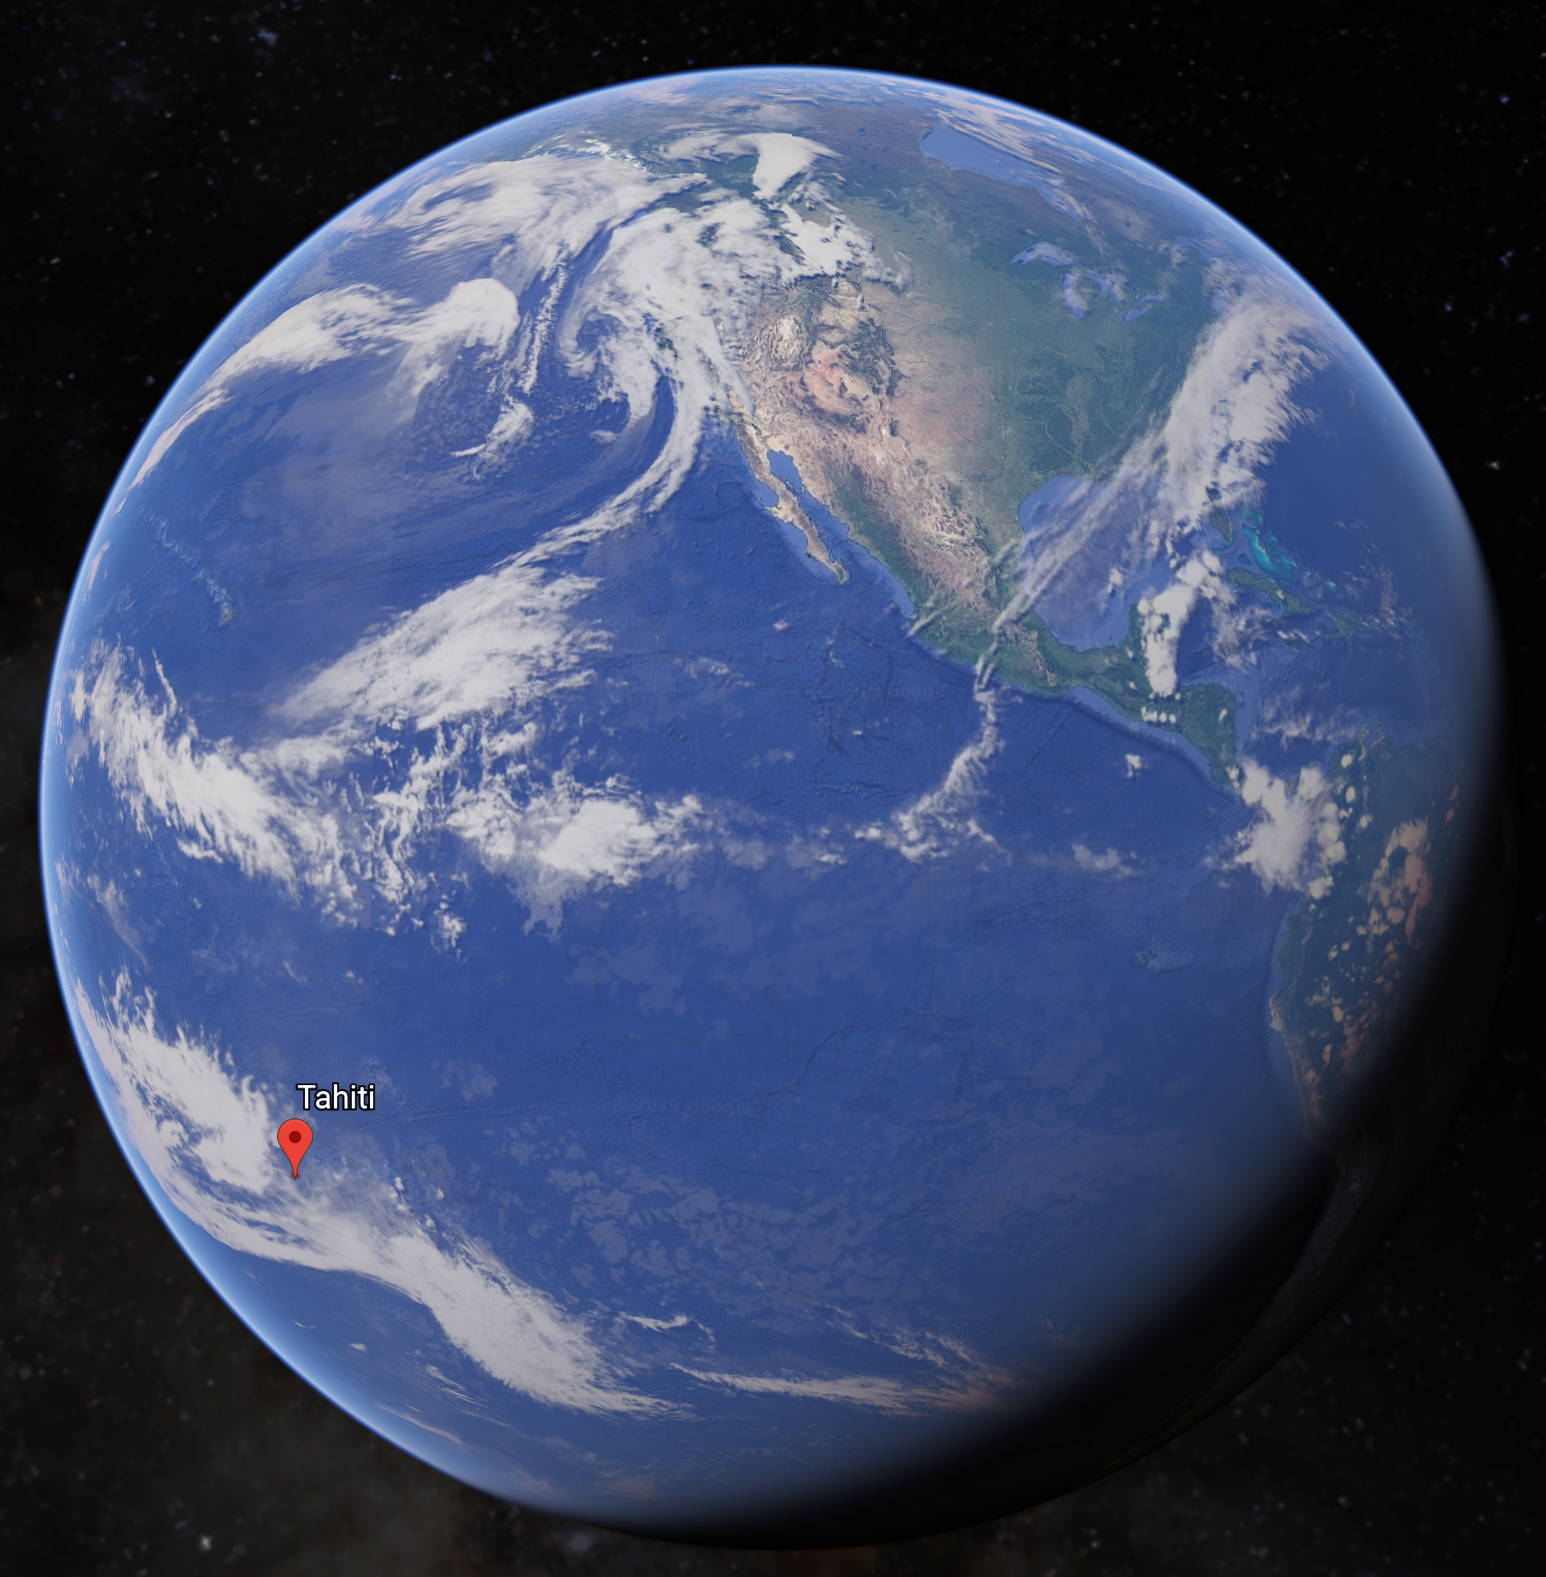
\includegraphics[height=5cm]{figures/tahitiloc.png}
		\label{tahitiloc}}
	\quad
	\subfloat[Tahiti from space]{
    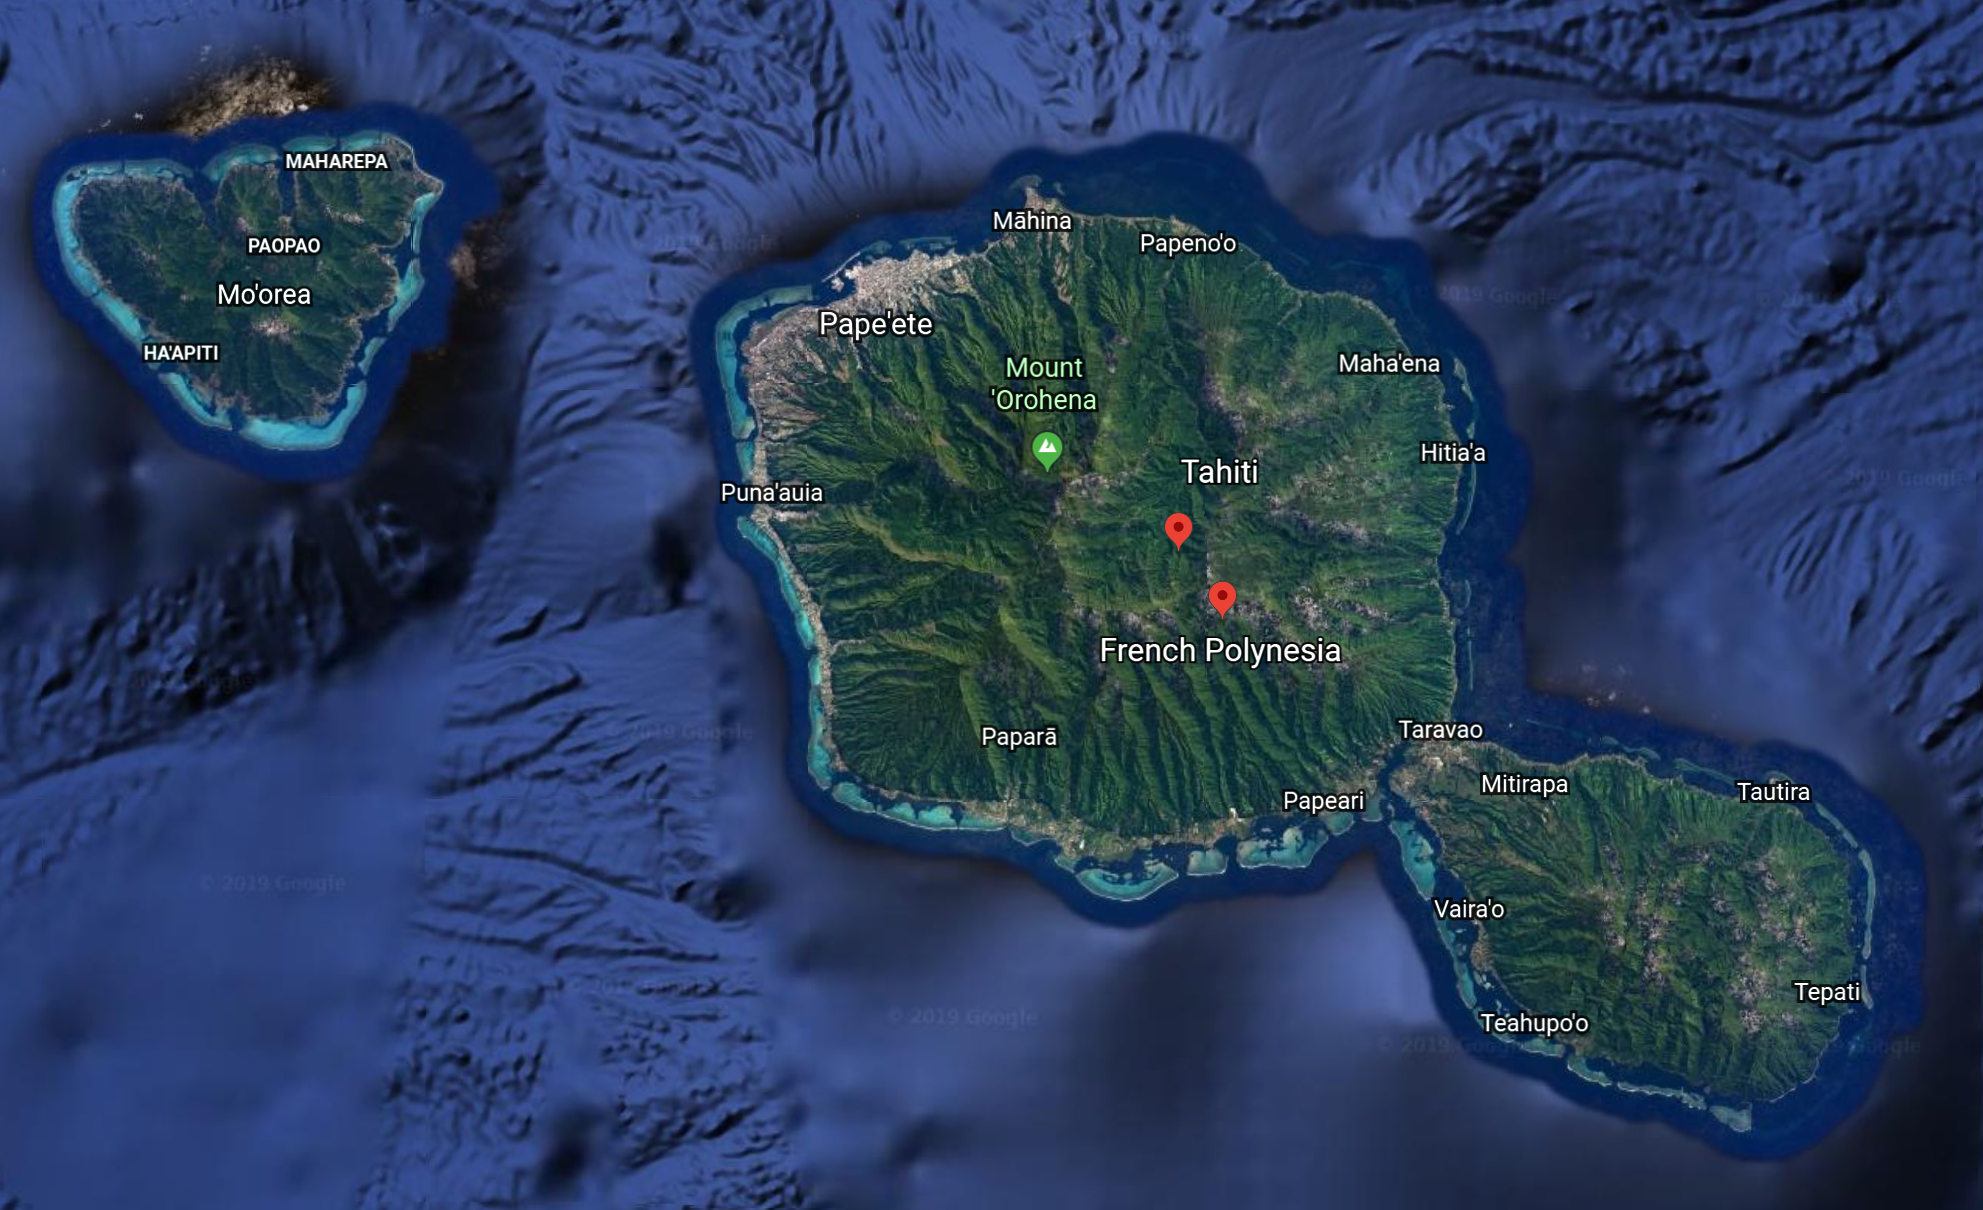
\includegraphics[height=5cm]{figures/tahitinear.png}
		\label{tahitinear}}
	\quad
	\caption{Tahiti's Location}
	\label{tahitilocation}
\end{figure}

\subsection{二级标题}

Subsection goes here. Sample Text.

The island is 45 km (28 mi) across at its widest point and covers an area of 1,045 km2 (403 sq mi). The highest peak is Mont Orohena (2,241 m (7,352 ft)). Mount Roonui, or Mount Ronui (Mou'a Rōnui), in the southeast rises to 1,332 m (4,370 ft). The island consists of two roughly round portions centered on volcanic mountains and connected by a short isthmus named after the small town of Taravao, which is situated there \cite{tahitiworldatlas}.

\begin{figure}[!h]
  \centering
  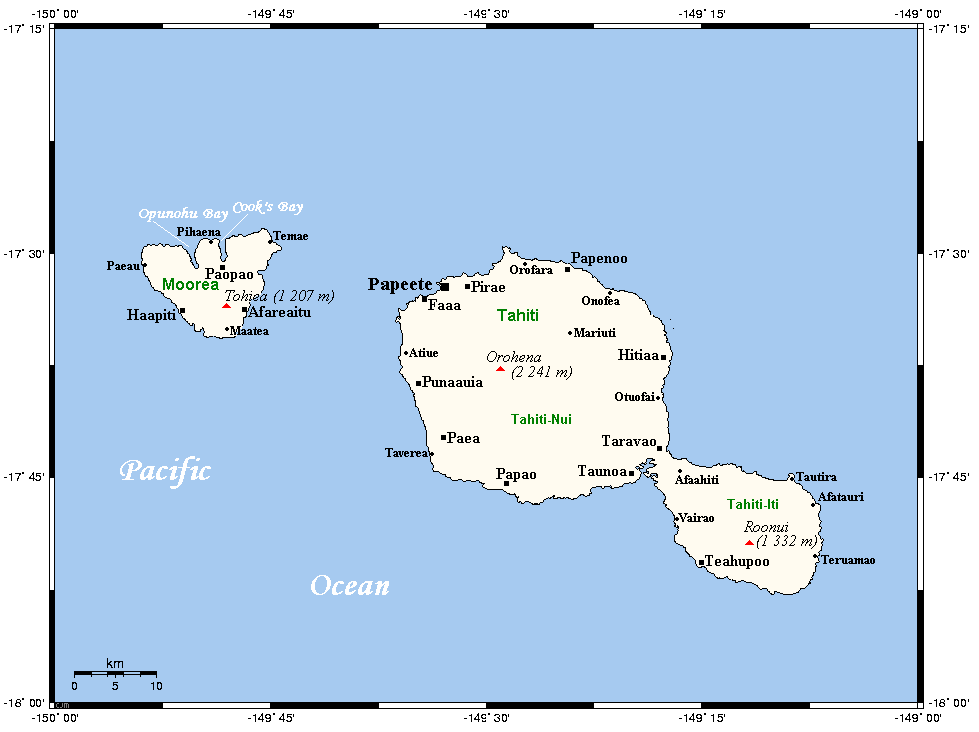
\includegraphics[height=6cm]{figures/TahitiMooreaMap.png}
  \caption{Tahiti Moorea Map}
  \label{tmmap}
\end{figure}

\subsubsection{三级标题}

Sub-subsection goes here, sample text.

Sample text.

\subsubsection{三级标题}

Sub-subsection goes here, sample text.

Sample text.

\section{一级标题}

Another Sample Section.

\section{结论}

Conclusion goes here.

%% Switch back default alignment of IEEE Template section title
\patchcmd{\section}{\raggedright}{\centering}{}{}
\patchcmd{\section}{\normalsize}{\large\bfseries}{}{}

\appendices
\section{Proof of the First Zonklar Equation}
Appendix one text goes here.

% % you can choose not to have a title for an appendix
% % if you want by leaving the argument blank
\section{}
Appendix two text goes here.


% % use section* for acknowledgment
\section*{致谢}

The authors would like to thank...

\ifCLASSOPTIONcaptionsoff
  \newpage
\fi

%% Comment below line out if you want references in a new page.
%\newpage

%% Citation files store in ref.bib
\bibliographystyle{IEEEtran}
% argument is your BibTeX string definitions and bibliography database(s)
\bibliography{IEEEabrv,ref}

%% Photos of Author, Comment out if you want add your personal information.
% \begin{IEEEbiography}{Michael Shell}
% Biography text here.
% \end{IEEEbiography}

% \begin{IEEEbiographynophoto}{Jane Doe}
% Biography text here.
% \end{IEEEbiographynophoto}

\end{document}


